\documentclass{standalone}
\usepackage{tikz}
\usetikzlibrary{patterns, positioning}

\begin{document}
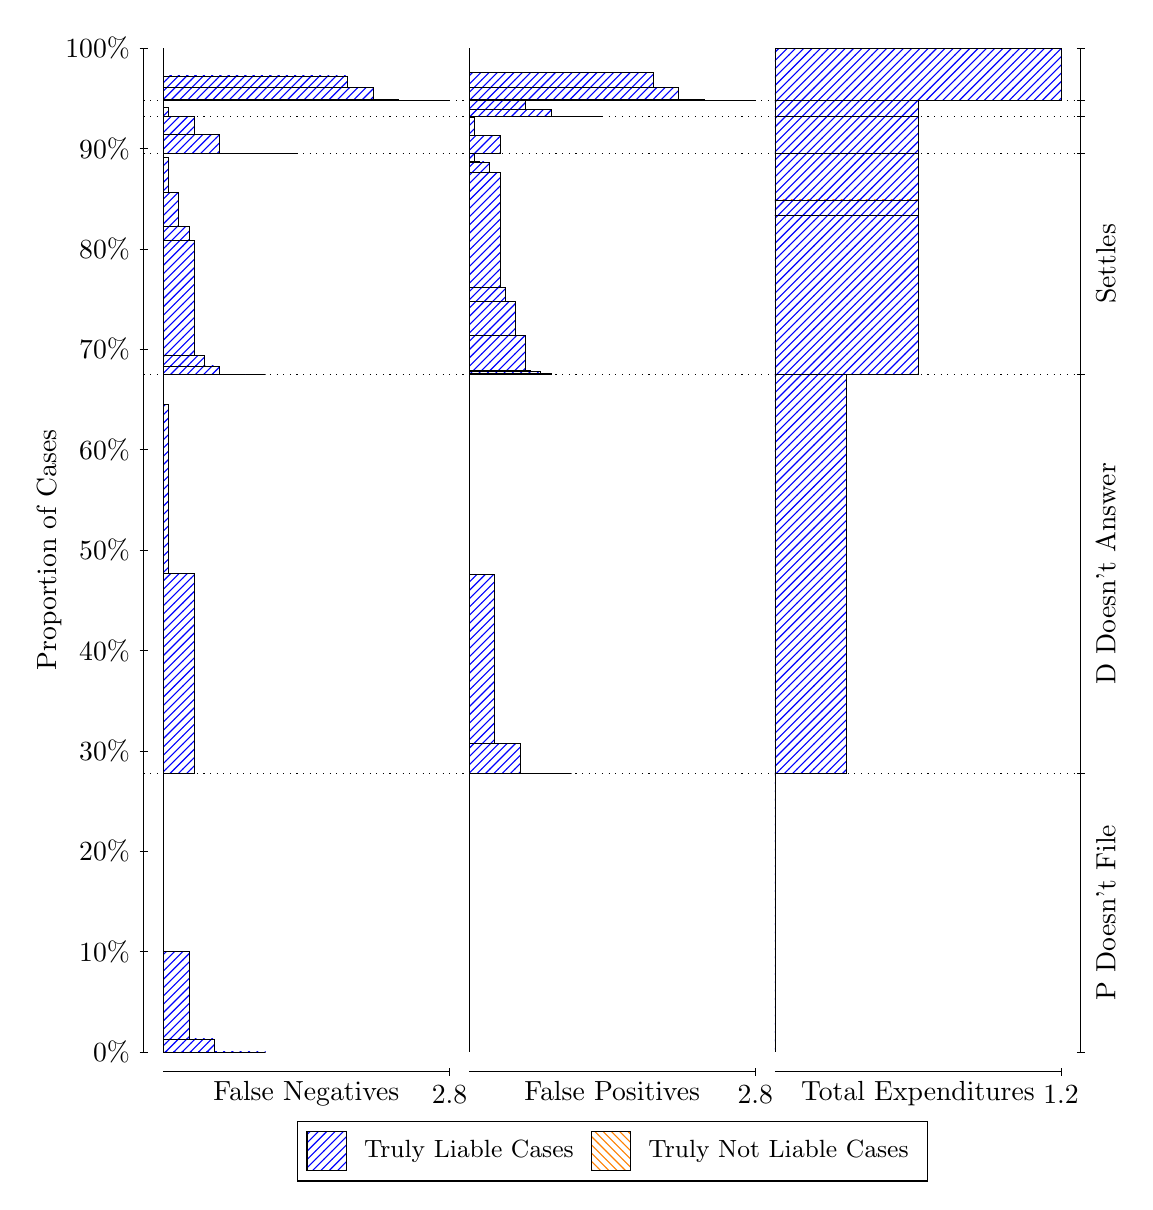
\begin{tikzpicture}
\draw[black, very thin] (1.5,1.75) -- (1.5,14.5);
\node[rotate=90, anchor=center] at (0.3, 8.125) {Proportion of Cases};
\draw[black, very thin] (1.45,1.75) -- (1.55,1.75);
\node[anchor=east] at (1.45, 1.75) {0\%};
\draw[black, very thin] (1.45,3.025) -- (1.55,3.025);
\node[anchor=east] at (1.45, 3.025) {10\%};
\draw[black, very thin] (1.45,4.3) -- (1.55,4.3);
\node[anchor=east] at (1.45, 4.3) {20\%};
\draw[black, very thin] (1.45,5.575) -- (1.55,5.575);
\node[anchor=east] at (1.45, 5.575) {30\%};
\draw[black, very thin] (1.45,6.85) -- (1.55,6.85);
\node[anchor=east] at (1.45, 6.85) {40\%};
\draw[black, very thin] (1.45,8.125) -- (1.55,8.125);
\node[anchor=east] at (1.45, 8.125) {50\%};
\draw[black, very thin] (1.45,9.4) -- (1.55,9.4);
\node[anchor=east] at (1.45, 9.4) {60\%};
\draw[black, very thin] (1.45,10.675) -- (1.55,10.675);
\node[anchor=east] at (1.45, 10.675) {70\%};
\draw[black, very thin] (1.45,11.95) -- (1.55,11.95);
\node[anchor=east] at (1.45, 11.95) {80\%};
\draw[black, very thin] (1.45,13.225) -- (1.55,13.225);
\node[anchor=east] at (1.45, 13.225) {90\%};
\draw[black, very thin] (1.45,14.5) -- (1.55,14.5);
\node[anchor=east] at (1.45, 14.5) {100\%};

\draw[black, very thin] (13.4,1.75) -- (13.4,14.5);
\draw[black, very thin] (13.35,1.75) -- (13.45,1.75);
\node[anchor=west] at (13.35, 1.75) {};
\draw[black, very thin] (13.35,5.287) -- (13.45,5.287);
\node[anchor=west] at (13.35, 5.287) {};
\draw[black, very thin] (13.35,10.357) -- (13.45,10.357);
\node[anchor=west] at (13.35, 10.357) {};
\draw[black, very thin] (13.35,13.161) -- (13.45,13.161);
\node[anchor=west] at (13.35, 13.161) {};
\draw[black, very thin] (13.35,13.63) -- (13.45,13.63);
\node[anchor=west] at (13.35, 13.63) {};
\draw[black, very thin] (13.35,13.837) -- (13.45,13.837);
\node[anchor=west] at (13.35, 13.837) {};
\draw[black, very thin] (13.35,14.5) -- (13.45,14.5);
\node[anchor=west] at (13.35, 14.5) {};

\draw[black, very thin, pattern color=blue, pattern=north east lines] (1.75,1.75) rectangle (3.0476,1.75);
\draw[black, very thin, pattern color=blue, pattern=north east lines] (1.75,1.75) rectangle (2.7232,1.7514);
\draw[black, very thin, pattern color=blue, pattern=north east lines] (1.75,1.7514) rectangle (2.3988,1.9173);
\draw[black, very thin, pattern color=blue, pattern=north east lines] (1.75,1.9173) rectangle (2.0744,3.0248);
\draw[black, very thin, pattern color=orange, pattern=north west lines] (1.75,3.0248) rectangle (1.75,3.0248);
\draw[black, very thin, pattern color=blue, pattern=north east lines] (1.75,3.0248) rectangle (1.75,5.287);
\draw[black, very thin, pattern color=blue, pattern=north east lines] (1.75,5.287) rectangle (2.1393,7.8329);
\draw[black, very thin, pattern color=blue, pattern=north east lines] (1.75,7.8329) rectangle (1.8149,9.9766);
\draw[black, very thin, pattern color=orange, pattern=north west lines] (1.75,9.9766) rectangle (1.75,9.9766);
\draw[black, very thin, pattern color=blue, pattern=north east lines] (1.75,9.9766) rectangle (1.75,10.357);
\draw[black, very thin, pattern color=blue, pattern=north east lines] (1.75,10.357) rectangle (3.0476,10.357);
\draw[black, very thin, pattern color=blue, pattern=north east lines] (1.75,10.357) rectangle (2.9179,10.357);
\draw[black, very thin, pattern color=blue, pattern=north east lines] (1.75,10.357) rectangle (2.7881,10.357);
\draw[black, very thin, pattern color=blue, pattern=north east lines] (1.75,10.357) rectangle (2.7232,10.357);
\draw[black, very thin, pattern color=blue, pattern=north east lines] (1.75,10.357) rectangle (2.5935,10.357);
\draw[black, very thin, pattern color=blue, pattern=north east lines] (1.75,10.357) rectangle (2.4637,10.456);
\draw[black, very thin, pattern color=blue, pattern=north east lines] (1.75,10.456) rectangle (2.3988,10.464);
\draw[black, very thin, pattern color=blue, pattern=north east lines] (1.75,10.464) rectangle (2.269,10.594);
\draw[black, very thin, pattern color=blue, pattern=north east lines] (1.75,10.594) rectangle (2.1393,12.061);
\draw[black, very thin, pattern color=blue, pattern=north east lines] (1.75,12.061) rectangle (2.0744,12.231);
\draw[black, very thin, pattern color=blue, pattern=north east lines] (1.75,12.231) rectangle (1.9446,12.668);
\draw[black, very thin, pattern color=blue, pattern=north east lines] (1.75,12.668) rectangle (1.8149,13.108);
\draw[black, very thin, pattern color=orange, pattern=north west lines] (1.75,13.108) rectangle (1.75,13.108);
\draw[black, very thin, pattern color=blue, pattern=north east lines] (1.75,13.108) rectangle (1.75,13.161);
\draw[black, very thin, pattern color=blue, pattern=north east lines] (1.75,13.161) rectangle (3.4369,13.161);
\draw[black, very thin, pattern color=blue, pattern=north east lines] (1.75,13.161) rectangle (3.1125,13.161);
\draw[black, very thin, pattern color=blue, pattern=north east lines] (1.75,13.161) rectangle (2.7881,13.166);
\draw[black, very thin, pattern color=blue, pattern=north east lines] (1.75,13.166) rectangle (2.4637,13.4);
\draw[black, very thin, pattern color=blue, pattern=north east lines] (1.75,13.4) rectangle (2.1393,13.63);
\draw[black, very thin, pattern color=orange, pattern=north west lines] (1.75,13.63) rectangle (1.75,13.63);
\draw[black, very thin, pattern color=blue, pattern=north east lines] (1.75,13.63) rectangle (2.1393,13.632);
\draw[black, very thin, pattern color=blue, pattern=north east lines] (1.75,13.632) rectangle (1.8149,13.746);
\draw[black, very thin, pattern color=orange, pattern=north west lines] (1.75,13.746) rectangle (1.75,13.746);
\draw[black, very thin, pattern color=blue, pattern=north east lines] (1.75,13.746) rectangle (1.75,13.837);
\draw[black, very thin, pattern color=blue, pattern=north east lines] (1.75,13.837) rectangle (5.3833,13.837);
\draw[black, very thin, pattern color=blue, pattern=north east lines] (1.75,13.837) rectangle (5.0589,13.837);
\draw[black, very thin, pattern color=blue, pattern=north east lines] (1.75,13.837) rectangle (4.7345,13.848);
\draw[black, very thin, pattern color=blue, pattern=north east lines] (1.75,13.848) rectangle (4.4101,14);
\draw[black, very thin, pattern color=blue, pattern=north east lines] (1.75,14) rectangle (4.0857,14.145);
\draw[black, very thin, pattern color=blue, pattern=north east lines] (1.75,14.145) rectangle (3.7613,14.146);
\draw[black, very thin, pattern color=blue, pattern=north east lines] (1.75,14.146) rectangle (3.4369,14.146);
\draw[black, very thin, pattern color=blue, pattern=north east lines] (1.75,14.146) rectangle (1.9446,14.146);
\draw[black, very thin, pattern color=orange, pattern=north west lines] (1.75,14.146) rectangle (1.75,14.146);
\draw[black, very thin, pattern color=blue, pattern=north east lines] (1.75,14.146) rectangle (1.75,14.5);
\draw[black, very thin, pattern color=orange, pattern=north west lines] (5.6333,1.75) rectangle (5.6333,1.75);
\draw[black, very thin, pattern color=blue, pattern=north east lines] (5.6333,1.75) rectangle (5.6333,5.287);
\draw[black, very thin, pattern color=orange, pattern=north west lines] (5.6333,5.287) rectangle (6.931,5.287);
\draw[black, very thin, pattern color=blue, pattern=north east lines] (5.6333,5.287) rectangle (6.931,5.287);
\draw[black, very thin, pattern color=blue, pattern=north east lines] (5.6333,5.287) rectangle (6.6065,5.289);
\draw[black, very thin, pattern color=blue, pattern=north east lines] (5.6333,5.289) rectangle (6.2821,5.6673);
\draw[black, very thin, pattern color=blue, pattern=north east lines] (5.6333,5.6673) rectangle (5.9577,7.811);
\draw[black, very thin, pattern color=blue, pattern=north east lines] (5.6333,7.811) rectangle (5.6333,10.357);
\draw[black, very thin, pattern color=orange, pattern=north west lines] (5.6333,10.357) rectangle (6.6714,10.357);
\draw[black, very thin, pattern color=blue, pattern=north east lines] (5.6333,10.357) rectangle (6.6714,10.368);
\draw[black, very thin, pattern color=orange, pattern=north west lines] (5.6333,10.368) rectangle (6.5417,10.368);
\draw[black, very thin, pattern color=blue, pattern=north east lines] (5.6333,10.368) rectangle (6.5417,10.393);
\draw[black, very thin, pattern color=orange, pattern=north west lines] (5.6333,10.393) rectangle (6.4119,10.393);
\draw[black, very thin, pattern color=blue, pattern=north east lines] (5.6333,10.393) rectangle (6.4119,10.411);
\draw[black, very thin, pattern color=blue, pattern=north east lines] (5.6333,10.411) rectangle (6.347,10.851);
\draw[black, very thin, pattern color=blue, pattern=north east lines] (5.6333,10.851) rectangle (6.2173,11.287);
\draw[black, very thin, pattern color=blue, pattern=north east lines] (5.6333,11.287) rectangle (6.0875,11.457);
\draw[black, very thin, pattern color=blue, pattern=north east lines] (5.6333,11.457) rectangle (6.0226,12.924);
\draw[black, very thin, pattern color=blue, pattern=north east lines] (5.6333,12.924) rectangle (5.8929,13.054);
\draw[black, very thin, pattern color=blue, pattern=north east lines] (5.6333,13.054) rectangle (5.7631,13.063);
\draw[black, very thin, pattern color=blue, pattern=north east lines] (5.6333,13.063) rectangle (5.6982,13.161);
\draw[black, very thin, pattern color=blue, pattern=north east lines] (5.6333,13.161) rectangle (5.6333,13.161);
\draw[black, very thin, pattern color=orange, pattern=north west lines] (5.6333,13.161) rectangle (6.0226,13.161);
\draw[black, very thin, pattern color=blue, pattern=north east lines] (5.6333,13.161) rectangle (6.0226,13.392);
\draw[black, very thin, pattern color=blue, pattern=north east lines] (5.6333,13.392) rectangle (5.6982,13.626);
\draw[black, very thin, pattern color=blue, pattern=north east lines] (5.6333,13.626) rectangle (5.6333,13.63);
\draw[black, very thin, pattern color=orange, pattern=north west lines] (5.6333,13.63) rectangle (7.3202,13.63);
\draw[black, very thin, pattern color=blue, pattern=north east lines] (5.6333,13.63) rectangle (7.3202,13.63);
\draw[black, very thin, pattern color=blue, pattern=north east lines] (5.6333,13.63) rectangle (6.9958,13.631);
\draw[black, very thin, pattern color=blue, pattern=north east lines] (5.6333,13.631) rectangle (6.6714,13.721);
\draw[black, very thin, pattern color=blue, pattern=north east lines] (5.6333,13.721) rectangle (6.347,13.835);
\draw[black, very thin, pattern color=blue, pattern=north east lines] (5.6333,13.835) rectangle (6.0226,13.837);
\draw[black, very thin, pattern color=orange, pattern=north west lines] (5.6333,13.837) rectangle (9.2667,13.837);
\draw[black, very thin, pattern color=blue, pattern=north east lines] (5.6333,13.837) rectangle (9.2667,13.837);
\draw[black, very thin, pattern color=orange, pattern=north west lines] (5.6333,13.837) rectangle (8.9423,13.837);
\draw[black, very thin, pattern color=blue, pattern=north east lines] (5.6333,13.837) rectangle (8.9423,13.837);
\draw[black, very thin, pattern color=orange, pattern=north west lines] (5.6333,13.837) rectangle (8.6179,13.837);
\draw[black, very thin, pattern color=blue, pattern=north east lines] (5.6333,13.837) rectangle (8.6179,13.847);
\draw[black, very thin, pattern color=orange, pattern=north west lines] (5.6333,13.847) rectangle (8.2935,13.847);
\draw[black, very thin, pattern color=blue, pattern=north east lines] (5.6333,13.847) rectangle (8.2935,14.001);
\draw[black, very thin, pattern color=blue, pattern=north east lines] (5.6333,14.001) rectangle (7.969,14.189);
\draw[black, very thin, pattern color=blue, pattern=north east lines] (5.6333,14.189) rectangle (7.6446,14.191);
\draw[black, very thin, pattern color=blue, pattern=north east lines] (5.6333,14.191) rectangle (7.3202,14.191);
\draw[black, very thin, pattern color=blue, pattern=north east lines] (5.6333,14.191) rectangle (6.9958,14.191);
\draw[black, very thin, pattern color=orange, pattern=north west lines] (5.6333,14.191) rectangle (5.6333,14.191);
\draw[black, very thin, pattern color=blue, pattern=north east lines] (5.6333,14.191) rectangle (5.6333,14.5);
\draw[black, very thin, pattern color=orange, pattern=north west lines] (9.5167,1.75) rectangle (9.5167,1.75);
\draw[black, very thin, pattern color=blue, pattern=north east lines] (9.5167,1.75) rectangle (9.5167,5.287);
\draw[black, very thin, pattern color=orange, pattern=north west lines] (9.5167,5.287) rectangle (10.425,5.287);
\draw[black, very thin, pattern color=blue, pattern=north east lines] (9.5167,5.287) rectangle (10.425,10.357);
\draw[black, very thin, pattern color=orange, pattern=north west lines] (9.5167,10.357) rectangle (11.333,10.357);
\draw[black, very thin, pattern color=blue, pattern=north east lines] (9.5167,10.357) rectangle (11.333,12.374);
\draw[black, very thin, pattern color=orange, pattern=north west lines] (9.5167,12.374) rectangle (11.333,12.374);
\draw[black, very thin, pattern color=blue, pattern=north east lines] (9.5167,12.374) rectangle (11.333,12.571);
\draw[black, very thin, pattern color=orange, pattern=north west lines] (9.5167,12.571) rectangle (11.333,12.571);
\draw[black, very thin, pattern color=blue, pattern=north east lines] (9.5167,12.571) rectangle (11.333,13.161);
\draw[black, very thin, pattern color=orange, pattern=north west lines] (9.5167,13.161) rectangle (11.333,13.161);
\draw[black, very thin, pattern color=blue, pattern=north east lines] (9.5167,13.161) rectangle (11.333,13.63);
\draw[black, very thin, pattern color=orange, pattern=north west lines] (9.5167,13.63) rectangle (11.333,13.63);
\draw[black, very thin, pattern color=blue, pattern=north east lines] (9.5167,13.63) rectangle (11.333,13.837);
\draw[black, very thin, pattern color=orange, pattern=north west lines] (9.5167,13.837) rectangle (13.15,13.837);
\draw[black, very thin, pattern color=blue, pattern=north east lines] (9.5167,13.837) rectangle (13.15,14.5);
\draw[black, dotted] (1.5,5.287) -- (13.4,5.287);
\draw[black, dotted] (1.5,10.357) -- (13.4,10.357);
\draw[black, dotted] (1.5,13.161) -- (13.4,13.161);
\draw[black, dotted] (1.5,13.63) -- (13.4,13.63);
\draw[black, dotted] (1.5,13.837) -- (13.4,13.837);
\draw[black, very thin] (1.75,1.5) -- (5.3833,1.5);
\node[anchor=north] at (3.5667, 1.5) {False Negatives};
\draw[black, very thin] (5.3833,1.45) -- (5.3833,1.55);
\node[anchor=north] at (5.3833, 1.45) {2.8};

\draw[black, very thin] (5.6333,1.5) -- (9.2667,1.5);
\node[anchor=north] at (7.45, 1.5) {False Positives};
\draw[black, very thin] (9.2667,1.45) -- (9.2667,1.55);
\node[anchor=north] at (9.2667, 1.45) {2.8};

\draw[black, very thin] (9.5167,1.5) -- (13.15,1.5);
\node[anchor=north] at (11.333, 1.5) {Total Expenditures};
\draw[black, very thin] (13.15,1.45) -- (13.15,1.55);
\node[anchor=north] at (13.15, 1.45) {1.2};

\node[black, centered, rotate=90] at (13.72, 3.5185) {P Doesn't File};
\node[black, centered, rotate=90] at (13.72, 7.8219) {D Doesn't Answer};
\node[black, centered, rotate=90] at (13.72, 11.759) {Settles};




\draw (7.449999999999999,1.5) node[draw=none] (baseCoordinate) {};
\begin{scope}[align=center]
        \matrix[scale=0.5, draw=black, below=0.5cm of baseCoordinate, nodes={draw}, column sep=0.1cm]{
            \node[rectangle, draw, minimum width=0.5cm, minimum height=0.5cm, pattern=north east lines, pattern color=blue] {}; &
            \node[draw=none, font=\small] (B) {Truly Liable Cases}; &
            \node[rectangle, draw, minimum width=0.5cm, minimum height=0.5cm, pattern=north west lines, pattern color=orange] {}; &
            \node[draw=none, font=\small] (B) {Truly Not Liable Cases}; \\
            };
\end{scope}

\end{tikzpicture}
\end{document}